\documentclass{article}
\usepackage{epsf}
\usepackage{graphicx}
\textwidth 6in
\textheight 9.5in
\topmargin -0.8in
\oddsidemargin 0in
\evensidemargin 0in
\parindent 0pt
\parskip 6pt

\begin{document}

\title{Physics 132\\
Amp\`ere's Law Exercise}
\maketitle


\bigskip\bigskip

Imagine an infinite plane, with charges flowing uniformly across it,
all in the same direction. You're going to find out what sort of
magnetic field is produced by such a ``current sheet.''\footnote{In
case you're wondering, there are actual systems like this in nature.
There aren't any \textit{infinite} current sheets, but in the outer
layers of the Sun, and in many other places, there are \textit{large}
current sheets, for which the results we'll get here provide quite a good
approximation.}

Here's one way to imagine an infinite current sheet. Imagine infinitely
many infinitely long straight wires, all placed right next to each other
in a plane. Each wire carries the same current $I$. This picture shows
a cross section of a bunch of those wires. Each one is carrying current
straight out of the page toward you. You should imagine that each wire
is infinite, and that they extend infinitely far to the left and right.
Let $n$ be the number of wires per unit meter.

\bigskip\bigskip

\centerline{
\includegraphics{figs/currentsheet.eps}}

\bigskip\bigskip

Our goal is to figure out the magnitude and direction of the magnetic field
at the location of the red dot.
Let's start with the direction. 

\begin{enumerate}
\item What is the direction of the magnetic
field at the red point, produced by the one wire that lies directly below
the dot?

\item Now consider one of the other wires,
say one that is five wires to the left of the dot.
What is the direction of the magnetic field at the red point produced by this 
wire? (You don't need to give me a precise angle here; just a sketch is fine.)

\item Now what about the wire that is five wires to the right of the dot?
What is the direction of the magnetic field at the red dot due to this wire?

\item If you added up the magnetic fields due to the wires in the two
previous questions, in which way would the resultant vector point?

\item If you added up the magnetic fields due to \textit{all} the wires,
which way would the resultant vector point?

The answer to the last question is the direction of $\vec B$ at 
the location of the red dot.

\item If you moved the red dot some distance to the left or right,
would the magnetic field change? Why not?

\item If you considered a point \textit{below} the wires instead of
above them, the same distance away as the red dot, what would the
direction of the magnetic field be?

Now let's go on to figure out the magnitude of the field.
Let $B$ stand for the as-yet-unknown magnitude of the field at the location of
the red dot. We're going to apply Amp\`ere's Law to the green loop in this
diagram:

\centerline{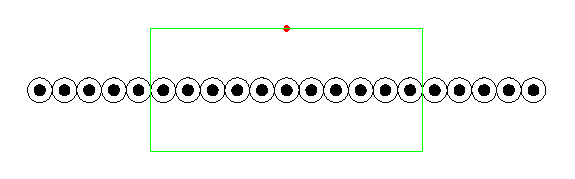
\includegraphics{figs/currentsheet2.eps}}

Let $L$ be the length of the green rectangle
and let $h$ be its height. 

\item How many wires are inside
the green rectangle? (Note: I don't want you just to count the
number in the picture; the picture's just an illustration. I want
an algebraic expression in terms of things like $n,L,h$.) 
How much total current is flowing through the 
interior of the green rectangle?

\item
Now evaluate the left side of Amp\`ere's Law, $\oint \vec B\cdot d\vec s$,
expressing the result in terms of some
or all of the quantities $B$ (which is what we're trying
to find), $L$, and $h$. In order to do this, you'll have to consider
the integral along each of the four sides of the rectangle,
and add them up.

\item In the last two questions, you worked out expressions
for the two sides of Amp\`ere's Law. Set them equal to each other
and solve for $B$.

We're done. That's the expression for the magnetic field produced 
by a current sheet.

\item Does the strength of the magnetic field depend on the
distance from the sheet?

\end{enumerate}

\end{document}







\end{document}
